\section{Introduction}
\label{sec:intro}

Die-to-die inspection compares each die with a reference die and flags where they differ. Most
differences are \emph{nuisance} (misalignment residue, linewidth variation, illumination), so a
second stage, the nuisance filter, decides which candidates are real defects. It is trained on
reviewed, labeled candidates, and labels are expensive: how many does it need?

This write-up builds such a pipeline on synthetic dies and compares what standard learning
theory says with what is measured, in four results: a VC bound for a threshold on peak contrast
(\cref{sec:result-1}); VC and Rademacher bounds for a linear filter (\cref{sec:result-2}); the
asymptotic learning curve of logistic regression, and its use to predict what more labels will
buy (\cref{sec:result-3}); and a certificate for the die-level false-alarm rate
(\cref{sec:result-4}). \Cref{sec:looseness} collects where the bounds lose. Every number below is
generated from a results file of the code.

\section{Setup}
\label{sec:setting}

\paragraph{Dies and stage 1.} A die is a $256\times256$ grayscale image of a product layout with
per-die nuisance (a smooth local warp that rigid alignment cannot remove, linewidth variation,
intensity blobs, line-edge roughness) and, on half of the dies, one defect (particle, scratch,
bridge, open or missing contact). Stage~1 aligns the die to a reference (the mean of
$\StageOneNReference$ defect-free dies) by FFT cross-correlation with sub-pixel refinement and a
least-squares gain/offset match, smooths $\abs{\text{test}-\text{reference}}$ with a Gaussian
($\sigma=1$\,px), thresholds it at $\tau=\StageOneTau$ and takes 8-connected components as
candidates. $\tau$ was tuned on $\StageOneNTune$ dies for recall $\StageOneTuningRecall$ (out of
sample: $\OvlRecall$). A candidate is a real defect ($y=+1$) iff it overlaps the defect mask.

\paragraph{Stage 2.} A threshold on peak contrast (Result~1), or a linear classifier
$x\mapsto\operatorname{sign}(w\cdot x)$ on $k$ features plus an intercept (Results~2--4). The
features are 10 hand-crafted ones (area, contrasts, shape, gradient energy, Laplacian of Gaussian
at two scales, distance to the nearest pattern edge) or a frozen ResNet-18 embedding of the
difference over the candidate ($d=384$), optionally reduced by PCA to 4, 16 or 64 dimensions. All
are standardized, clipped and rescaled so $\norm{x}\le C=1$. A die is flagged at threshold $t$ iff
some candidate's score exceeds $t$.

\paragraph{Sampling.} Candidates on one die are dependent, so each example is one candidate drawn
uniformly from a freshly generated die (dies without candidates are redrawn). With $D$ a random
die and $C(D)$ its candidates, examples are i.i.d.\ from
\[
  Q(A)=\frac{\E\bigl[\,\abs{C(D)\cap A}/\abs{C(D)}\;;\;\abs{C(D)}\ge1\bigr]}{\P(\abs{C(D)}\ge 1)}.
\]
Candidate-level error rates are probabilities under $Q$, which gives each die weight 1, so they
are not die-level rates; only Result~4 is a die-level statement. The positive rate under $Q$ is
$\pi=\OvlPositiveRate$ ($\OvlCandPerDie$ candidates per die), so the trivial classifier errs
$\min(\pi,1-\pi)=\TrivialError$; a bound on the 0-1 error says something only below that.

\paragraph{Pools and regimes.} All data come from separately seeded pools, and every choice is
made on the validation pool. Two regimes differ only in defect contrast. In the \emph{separable}
one the best threshold on peak contrast makes $\SepBestErrors$ errors on $\SepNPopulation$
candidates; in the \emph{overlapping} one, the main setting, it errs $\OvlBestErrorRate$
(\cref{fig:regimes}). All results use $\delta=0.05$.

\begin{center}
\small
\begin{tabular}{llr}
\toprule
pool & used for & size used \\
\midrule
feature-fit / validation & PCA, scaling / every choice ($B$, grid) & $\PoolFeatureFit$ / $\PoolValidation$ candidates \\
train & a fresh block per repeat & up to $\PoolTrainEThreeB$ candidates \\
population / test & $L(h^\star)$, $\theta^\star$ / measured errors, $H$, $G$ & $\PoolPopulationEThree$ / $\PoolTest$ candidates \\
certification / far-test & Result~4, defect-free dies & $\PoolCertification$ / $\PoolFarTest$ dies \\
\bottomrule
\end{tabular}
\end{center}

\begin{figure}[tb]
  \centering
  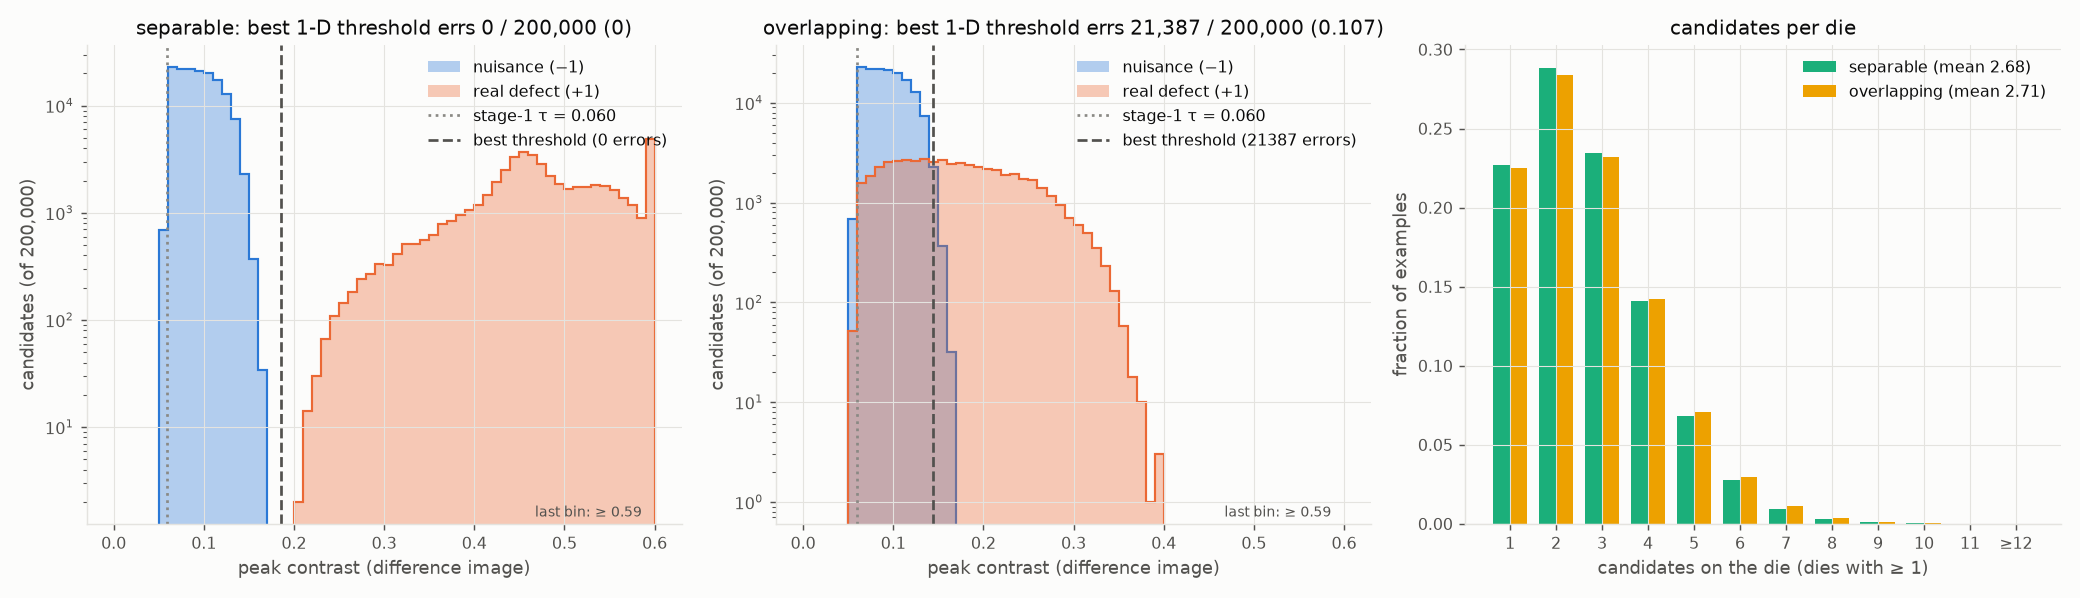
\includegraphics[width=0.8\linewidth]{../figures/stage1_regimes.png}
  \caption{Peak contrast of nuisance and real-defect candidates in the two regimes (population
  pool) and candidates per die.}
  \label{fig:regimes}
\end{figure}
